%% 
%% Author:  Olivier Fourmaux (olivier.fourmaux@upmc.fr)
%% 


%%%%%%%%%%%%%%%%%%%%%%%%%%%%%%%%%%%%%%%%%%%%%%%%%%%%%%%%%%%
%% Type et package

\documentclass[a4paper,12pt]{article}

\usepackage[francais,english]{babel}
\usepackage{fancyhdr}
\usepackage[latin1]{inputenc}
\usepackage{epsfig}
\usepackage{calc}
\usepackage{url}
\usepackage{boxedminipage}

%%%%%
%%Rajout
\input{formatanddefs}



%%%%%%%%%%%%%%%%%%%%%%%%%%%%%%%%%%%%%%%%%%%%%%%%%%%%%%%%%%%
%%%%%%%%%%%%%%%%%%%%%%%%%%%%%%%%%%%%%%%%%%%%%%%%%%%%%%%%%%%
%% D�finitions � personnaliser 

%% Pour les noms, utilisez la premi�re lettre du pr�nom suivi du 
%% nom de famille (premi�re lettre majuscule, reste en minuscule).


%%%% Indiquer le nom de l'encadrant ci-dessous:

\def\nomEncad{S.~Secci,\\ Y.~Bencha�b, M.~Coudron}
%%<matthieu.coudron@lip6.fr>,
%%<yacine.benchaib@lip6.fr>
%% Si le projet est co-encadr� indiquer les deux noms � la suite dans 
%% Le m�me champs


%%%% Indiquer les noms des �tudiants participant ci-dessous:

\def\nomEtudC{Q.~Dubois}
\def\nomEtudB{K.~Lam}
\def\nomEtudA{R.~Ly}
\def\nomEtudD{S.~Ravier}

%% Si le projet est encadr� par moins de 4 �tudiants laissez
%% les variables inutiles vides


%%%% Indiquer la r�f�rence (numero) et le nom du sujet ci-dessous:

\def\refProjet{9} \def\titreProjetCourt{perf\,MPTCP\,OpenFlow}
\def\titreProjetLong{MPTCP\\Performances et optimisation de la
  s�curit� avec un ordonnancement r�parti dans les topologies
  virtualis�es OpenFlow}

%% Le titre court ne doit pas faire plus d'une vingtaine de caract�re
%% r�sumez le � quelques mots essenciels


%%%% Indiquer le type de document et sa version ci-dessous:

\def\typeDoc{Rapport final}
 
%% - Rapport interm�daire
%% - Rapport final



%%%%%%%%%%%%%%%%%%%%%%%%%%%%%%%%%%%%%%%%%%%%%%%%%%%%%%%%%%%
%%%%%%%%%%%%%%%%%%%%%%%%%%%%%%%%%%%%%%%%%%%%%%%%%%%%%%%%%%%
%% D�finitions � ne pas modifier
 
%%%%% ||| Mise en page verticale ||| 
\setlength{\voffset}{-1in} % a4:reste 297mm pour les 5 suivants:
\setlength{\topmargin}{15mm}         % avant l'en-t�te
\setlength{\headheight}{20mm}        % hauteur de l'en-t�te 
\setlength{\headsep}{10mm}            % entre l'en-t�te et le corps
\setlength{\textheight}{220mm}       % hauteur du corps
\setlength{\footskip}{12mm}          % pied de page par rapport au corps 

%%%%% --- Mise en page horizontale ---
\setlength{\hoffset}{-1in} % a4:reste 210mm 
\setlength{\oddsidemargin}{25mm}     % entre hoffset et le corps
\setlength{\evensidemargin}{25mm}    % entre hoffset et le corps
\setlength{\marginparwidth}{0mm}     % largeur de la marge
\setlength{\marginparsep}{0mm}       % s�parateur corps marge
\setlength{\textwidth}{160mm}        % largeur du corps

\def\annee{2013-14}



%%%%%%%%%%%%%%%%%%%%%%%%%%%%%%%%%%%%%%%%%%%%%%%%%%%%%%%%%%%
%% D�but du document

\begin{document}

\selectlanguage{francais}



%%%%%%%%%%%%%%%%%%%%%%%%%%%%%%%%%%%%%%%%%%%%%%%%%%%%%%%%%%%
%% D�finition des en-t�tes et pied de pages
\pagestyle{fancyplain}
\lhead[\fancyplain{}{\texttt{Universit� Pierre et Marie Curie}\\
          Master Informatique\\ UE \textbf{PRes} f�v. \annee \\ \nomEncad}]
      {\fancyplain{}{\textsc{Universit� Pierre et Marie Curie}\\
          Master Informatique\\ UE \textbf{PRes} \annee \\ \nomEncad}}
\chead[\fancyplain{}{\textbf{Projet \refProjet\\\titreProjetCourt}}]
      {\fancyplain{}{\textbf{Projet \refProjet\\\titreProjetCourt}}}
\rhead[\fancyplain{}{\nomEtudA\\\nomEtudB\\\nomEtudC\\\nomEtudD}]
      {\fancyplain{}{\nomEtudA\\\nomEtudB\\\nomEtudC\\\nomEtudD}}
\lfoot[\fancyplain{}{\epsfig{figure=UPMC_sorbonne.eps,width=3cm}}]
      {\fancyplain{}{\epsfig{figure=UPMC_sorbonne.eps,width=3cm}}}
\cfoot[\fancyplain{}{\textbf{\thepage/\pageref{fin}}}]
      {\fancyplain{}{\textbf{\thepage/\pageref{fin}}}}
\rfoot[\fancyplain{}{\typeDoc}]
      {\fancyplain{}{\typeDoc}}

%%%%%%%%%%%%%%%%%%%%%%%%%%%%%%%%%%%%%%%%%%%%%%%%%%%%%%%%%%%

~

      \begin{center}
        \begin{boxedminipage}{12cm}{
            \begin{center}
              ~\\\LARGE\textbf{\titreProjetLong}\\
              ~\\\large Encadrants: \textbf{\nomEncad,}\\
              ~\\\large Etudiants: \textbf{\nomEtudA, \nomEtudB, \nomEtudC, \nomEtudD}\\
              ~
            \end{center}
            }
        \end{boxedminipage}
      \end{center}

~

\tableofcontents

\section{Cahier des charges}

\subsection{Objectifs}
\label{sec:charges:intro}

Les objectifs du projet sont de 
\begin{itemize}
\item mesurer les performances de MPTCP sur diff�rentes topologies de
  r�seaux virtuels.
\item modifier l'ordonnanceur de MPTCP pour privili�ger une
  r�partition �quilibr�e sur les diff�rents sous-flots.
\end{itemize}

\subsection{Contexte}
\label{sec:charges:contexte}

MPTCP est une extension de TCP qui permet pour une connexion TCP
donn�e d'utiliser plusieurs chemins pour l'�change de donn�es. La
multiplicit� des sous-flots a pour but d'am�liorer le d�bit et
d'augmenter la r�silience de la connexion\cite{rfc6182,rfc6824,
  coudroncross2013}.

L'utilisation de MPTCP ne doit en aucun cas diminuer les performances
de l'utilisateur en dessous des performances d'une simple connexion
TCP ou diminuer le d�bit des autres utilisateurs sur le m�me
r�seau. Les performances de MPTCP d�pendent en partie de l'algorithme
utilis� pour la r�partition des donn�es entre les diff�rents
sous-flots ouverts \cite{pareto2013}. Pour caract�riser les
performances de l'ordonnanceur de MPTCP, nous allons le tester dans
diff�rents r�seaux virtualis�s en utilisant dans un premier temps
l'algorithme par d�faut.

L'utilisation exclusive d'un chemin dans une connexion TCP permet la
possibilit� � un attaquant d'�couter la totalit� des donn�es
�chang�es, d'utiliser des attaques de type rejeu ou \emph{man in the
  middle}.  L'emploi de MPTCP am�liorerait la s�curit� si les donn�es
transitaient de mani�re �quilibr�e entre les diff�rents sous-flots. Le
d�bit global de la connexion serait affect� car les chemins les plus
lents vont ralentir le d�bit des chemins les plus rapides. Nous
allons, dans un premier temps, modifier l'ordonnanceur afin de
garantir la r�partition �quitable des charges au d�triment du d�bit
puis analyser l'influence de cette modification sur les performances
de MPTCP dans les topologies r�seaux utilis�s pr�c�demmment. Si nous
avons le temps, nous r�fl�chirons s'il est possible d'obtenir un
algorithme pouvant garantir une s�curit� et un d�bit sup�rieur � celle
d'une simple connexion TCP pour que cela soit conforme aux objectifs
premiers de MPTCP.

\subsection{M�thodes}
\label{sec:charges:methodes}

La simulation des r�seaux sera effectu� via mininet qui va nous
permettre de simuler un r�seau OpenFlow. Pour caract�riser l'influence
de l'ordonnanceur sur les performances, nous utiliserons des r�seaux
simples o� les diff�rents sous-flots sont asym�triques et diff�rent
par une propri�t� � la fois: latence, d�bit, pertes ...\\

Nous testerons diff�rents algorithmes de r�partition de charge entre
les sous-flots: l'algortihme impl�ment� par d�faut (LIA), celui qui
satisfait l'optimum de pareto par rapport aux objectifs de MPTCP
(OLIA, \cite{pareto2013}) ou celui qu'on va d�velopper qui permet de
r�partir de mani�re �quilibr�� les charges dans les diff�rents
sous-flots.

Nous utiliserons des scripts python pour automatiser la cr�ation des
sous-flots ainsi que les tests de performance.\\

Pour impl�menter l'algorithme de balancement �quilibr� (favorisant la
s�curit�), nous modifierons le code source de MPTCP:
\url{https://github.com/multipath-tcp/mptcp/tree/mptcp_v0.88/net/mptcp}.
Dans un premier temps,
\begin{itemize}
\item nous privil�gierons une r�partition �quitable entre les
  diff�rents sous-flots.
\item il est aussi n�cessaire de g�rer les probl�mes li�s � la
  retransmission, pour �viter que les paquets soient r�exp�di�s sur le
  m�me sous-flot en cas de congestion ou de panne d'un sous-flot, qui
  dans ce cas renderait l'avantage de l'agorithme nulle.
\item et ensuite mesurer les performances de notre algorithme.
\end{itemize}

\subsection{R�partition}
\label{sec:charges:repartition}

Nous allons r�partir la charge de travail en deux groupes de deux
personnes. Le premier groupe va �difier les r�seaux virtuels ainsi que
les outils d'analyses. Le deuxi�me groupe personnes s'occupera du code
de l'ordonnanceur sans exclure l'aide ou la concertation entre les
deux groupes.

%// -*- coding: iso-8859-1 -*-
\section{Plan de d\'eveloppement}
\label{sec:plan:devt}

La premi�re partie est de consuitre les topologies virtualis�es et de
tester les performances de MTPCP en faisant varier les param�tres des
sous-flots. La seconde partie est de construire un alogrithme
d'ordonnancement r�pondant � des crit�res de s�curit�.
\vspace{0.5cm}

Les �tapes du d�veloppement suivront les points suivants:

\begin{itemize}
\item Pr�paration d'une machine mininet avec le noyau MPTCP compil�
  pour l'ensemble de l'�quipe:
\item Lecture, compr�hension et commentaires du code de MPTCP;
\item Pr�paration de plusieurs topologies : \emph{fat tree} pour
  simuler un \emph{data center} et une topologie permettant de tester
  la concurrence entre MPTCP et TCP;
\item Pr�paration d'une biblioth�que de tests et de mesures via l'API python;
\item \'Ecriture d'un algorithme d'ordonnancement dans le noyau;
\item Mesures de performance des diff�rents algorithmes.
\end{itemize}




\begin{figure}[!htb]
  \begin{changemargin}{-2.0cm}{0.5cm}
    \centering
    \includegraphics[width=1.2\textwidth]{../gantt/gant.jpg}
  \end{changemargin}
  \centering
  
  \caption{\textbf{Diagramme de Gantt g�n�ral}. Les couleurs
    correspondent � la r�partition entre les membres de l'�quipe : en
    \emph{rouge} M. Ly, en \emph{jaune} M. Ravier et en \emph{vert}
    M. Dubois et M. Lam, en \emph{orange} M. Ravier et M. Ly et en
    \emph{noir} par tout le monde.}
  \label{fig:gantt}
  
\end{figure}

\vspace{2cm}

\begin{figure}[!htb]
  \begin{changemargin}{-2.0cm}{0.5cm}
    \centering
    \includegraphics[width=1.2\textwidth]{../gantt/romain.jpg}
  \end{changemargin}
  \centering
  
  \caption{\textbf{Diagramme de Gantt personnalis�e Romain Ly.}}
  \label{fig:gantt}
  
\end{figure}

\begin{figure}[!htb]
  \begin{changemargin}{-2.0cm}{0.5cm}
    \centering
    \includegraphics[width=1.2\textwidth]{../gantt/kevin.jpg}
  \end{changemargin}
  \centering
  
  \caption{\textbf{Diagramme de Gantt personnalis�e Kevin Lam et
      Quentin Dubois.}}
  \label{fig:gantt}
  
\end{figure}



\clearpage
\section{Contexte technologique}
\label{sec:contexte-techno}
%// -*- coding: iso-8859-1 -*-

L'�laboration de MPTCP a �t� motiv�e par l'observation de l'existence
dans les r�seaux de plusieurs chemins entre deux machines A et
B. L'utilisation de ces diff�rents chemins entre les deux h�tes
pourrait �tre un atout non n�gligeable pour augmenter le d�bit de la
connexion et/ou la r�silience de la connexion si l'un des chemins
venait � ne plus pouvoir acheminer les paquets (congestion, panne de
routeur, etc). De plus le multi-chemin permet d'�quilibrer la
r�partition des charges sur les sous-flots utilis�s. TCP n'a pas �t�
con�u pour exploiter plusieurs chemins d'o� la n�cessit� de concevoir
des protocoles multi-chemins comme MPTCP permettant d'utiliser les
chemins disponibles pour transmettre les paquets d'une connexion entre
A et B via les sous-flots connect�s.

Il existe d�j� plusieurs protocoles proposant d'utiliser plusieurs
chemins. Nous en citerons que deux: SCTP et ECMP. SCTP (\emph{Stream
  Control Transmission Protocol}) allie l'avantage de TCP et UDP et
permet de multiplexer les flux sur plusieurs interfaces
\cite{rfcsctp}. ECMP (\emph{Equal Cost MultiPath}) est un protocole
qui semblait prometteur dans les data center. Lors d'une connexion
entre deux h�tes, le routeur peut transf�rer les paquets sur plusieurs
meilleurs chemins � co�ts \og �gaux \fg{}
\cite{rfcecmp}. L'inconv�nient de SCTP est la n�cessit� que tous les
h�tes terminaux puissent comprendre le protocole ; il est donc
n�cessaire de modifier la couche application pour pouvoir
l'utiliser. ECMP n�cessite le travail des routeurs pour conna�tre les
chemins et l'augmentation de performance n'est pas forc�ment
significative. L'avantage de MPTCP est d'�tre transparent par rapport
� TCP, c'est � dire que si un h�te n'est pas compatible avec MPTCP, la
connexion retournera vers une connexion TCP classique. L'autre
avantage est qu'il est totalement transparent pour les routeurs, c'est
une connexion \emph{end to end}.


\subsection{Fonctionnement de MPTCP}
\label{subsec:fonctMPTC}

MPTCP utilise dans un premier temps une connexion TCP pour cr�er des
sous-flots similaire � TCP avec des chemins diff�rents. La couche TCP
est alors remplac�e par la couche MPTCP qui est divis�e en deux
parties : la couche sup�rieure correspond aux fonctions n�cessaires �
MPTCP de fonctionner (d�couverte et gestion des chemins,
ordonnancement des paquets, contr�le de congestion) et la couche
inf�rieure correspond aux sous-flots �tablis.

Lorsque MPTCP utilise plusieurs sous-flots (si les chemins diff�rents
existent), le d�bit est augment� de mani�re � ce qu'il soit sup�rieur
� une connexion TCP unique sur le meilleur des chemins utlis�s. MPTCP
augmente aussi la r�silience de la connexion, si un sous-flot est
congestionn�, le traffic est alors r�parti et/ou r�exp�di� sur les
autres sous-flots sans qu'il y a it besoins de r�tablir une connexion
MPTCP entre les deux terminaux. Cette approche permet d'utiliser les
ressources disponibles par une approche bout en bout.

Mais pour pouvoir profiter de ces deux avantages, le gestionnaire des
chemins est essentiel car c'est en d�couvrant de multiples chemins,
s'il en existe, que la r�silience, la r�sistance aux pannes et le
d�bit sont accrus. Il permet de d�couvrir de nouveaux sous-flots, les
supprimer en cas de panne d'un sous-flot ou si celui-ci est beaucoup
trop lent (car cela ralentirait le d�bit global de MPTCP).

L'ordonnanceur des paquets, quant � lui, est �galement utile pour
cette augmentation en d�bit. En effet, c'est la fonction qui permet de
g�rer les diff�rents buffers des sous-flots, d'organiser le nombre de
paquets � envoyer dans chaque sous-flot et de modifier cette quantit�,
en cas de n�cessit�.  C'est ce qui permet d'utiliser de fa�on
synchrone plusieurs sous-flots TCP.

\vspace{0,5cm}
Enfin, le contr�le de congestion est un outil pour les deux fonctions
pr�c�dentes. C'est la fonction qui permet d'adapter le d�bit de chaque
sous-flot et de d�finir si un chemin est trop lent par rapport au
meilleur sous-flot, ce qui est une optimisation. Il permet aussi de
renvoyer l'information au gestionnaire s'il y a une panne.

Le contr�le de congestion n�cessite un algorithme performant pour que
l'utilisation de MPTCP � la place de TCP puisse effectivement
augmenter le d�bit de l'utilisateur sans influencer le d�bit des
autres utilisateurs sur les m�mes chemins, c'est � dire qu'il doit
garantir l'optimalit� de pareto. L'algorithme de MPTCP est donc un
point central dans les performances de MPTCP sur le r�seau.

Lors des choix des sous-flots, l'algorithme doit effectuer un
compromis entre �quilibre des charges dans les diff�rents sous-flots
et r�activit� (\emph{responsiveness}) en cas de modification de la
latence des sous-flots ou de d�couvertes de nouveaux chemins. Une
priorit� vers l'�quilibre des charges entra�ne l'envoi des donn�es sur
les meilleurs routes (selon la m�trique utilis�e, par d�faut la
latence du chemin) mais peut d�clencher un changement constant de
route produisant un effet de battement (\emph{flappiness}): si
plusieurs chemins poss�dent le m�me co�t, l'algorithme aura tendance �
changer tr�s souvent de chemins. Si la priorit� utilis�e est la
r�activit� (par exemple augmentation de la taille de la fen�tre d'un
des sous-flot), l'utilisation de toutes les ressources disponibles
peut ne pas �tre optimale car on aura tendance � utiliser qu'un seul
sous-flot. Les param�tres de l'algorithme doit �tre d�terminer
efficacement pour �quilibrer les charges sur les sous-flots et ne pas
�tre agressif (augmentation trop rapide de la taille de la fen�tre
sur un des sous-flots) pour garantir l'optimalit� de Pareto.

 Dans l'algorithme par d�faut, le crit�re privili�g� par l'algorithme
est le RTT. Il serait int�ressant de modifier les caract�ristiques du
r�seau pour mesurer les performance de MPTCP sur le choix des chemins
utilis�es ou en cas de modification du chemins sur des crit�res de
latence, pertes, d�bit \ldots



\subsection{Utilisation r�elle de MPTCP}
\label{subsec:utilisation}

Dans la pratique, l'utilisation de MPTCP est difficile. L'utilisation
de plusieurs sous-flots ne garantie pas l'augmentation de d�bit. Pour
cel�, il est n�cessaire que les sous-flots empruntent des chemins
physiques diff�rents et aujourd'hui il n'est pas possible pour un
utilisateur de contr�ler le routage de ses paquets de bout en
bout. Une m�thode pour contourner le probl�me serait d'utiliser la
conjonction de MPTCP et de LISP (\emph{Locator/Identifier Separation
  Protocol}) qui permet de d�couvrir la diversit� de chemins existant
entre routeurs de bordures (A-MPTCP)
\cite{coudroncross2013}. 

Cependant il existe des cas o� MPTCP est utilisable � son plein
potentiel et suscite l'int�r�t : dans les data center et en
utilisation mobile. Par l'int�rm�diaire d'une strat�gie de routage par
SDN (\emph{Software Defined Network}) par exemple openFlow, le
contr�leur peut �tablir des chemins diff�rents entre deux h�tes sur
tout son r�seau. Le transfert de donn�es au sein d'un data center
n�cessite des d�bits tr�s importants. L'utilisation de MPTCP pourrait
�quilibrer les charges entre les diff�rents noeuds. Des exp�riences
sur diff�rents topologies de data center denses ont permis de montrer
que MPTCP �gale et surpasse m�me la performance d'un ordonnanceur
centralis� et est de surcroit plus robuste \cite{raiciu2010}. En
mobile, le terminal pourra utiliser le r�seau 3G/4G et le r�seau wi-fi
environnant. MPTCP permettra de d�charger le r�seau t�l�phonique de
l'op�rateur tout en augmentant le d�bit et la r�silience de la
connexion.

\subsection{MPTCP et s�curit�}
\label{subsec:utilisation}

\`A l'heure d'Eric Snowden, l'utilisation de plusieurs sous-flots
pourrait �tre un avantage non n�gligeable en terme de s�curit�. Pour
pouvoir �pier une connexion entre A et B, il faudrait � l'attaquant de
pouvoir \emph{sniffer} les paquets qui sont �mis sur les sous-flots
utilis�s, c'est � dire sur autant de chemins physiques
diff�rents. L'int�r�t du multi-chemin prend alors tout son
sens. Cependant ce n'est pas le seul avantage.

L'utilisation de chiffrement de type CBC (\emph{Cipher Block
  Chaining}) compliquera l'attaquant car il est n�cessaire d'avoir le
bloc n-1 pour d�chiffrer le bloc n. AES-CBC est utilis� couramment
dans des communications de type HTTPS/SSL. Il sera n�cessaire �
l'attaquant de disposer de tous les paquets sans exception pour
pouvoir d�chiffrer le message en supposant qu'il poss�de la cl�
ad�quate.

De plus, si les protocoles de s�curit� sont conscients de
l'utilisation de MPTCP, il pourrait y avoir une entente
\emph{cross-layer}. Par exemple, en distribuant les informations des
MAC (\emph{Message Authentication Code}) de chaque paquet entre les
diff�rents sous-flots de mani�re � �viter les \emph{man in the
  middle}: sous flot 1 = message 1 + HMAC (message 2); sous flot 2 =
message 2 + HMAC (message 1).  Un autre exemple serait de n�gocier les
cl�s pour le chiffrement de la communication d'un sous-flot (par
exemple en utilisant IPSec) dans le sous-flot adjacent.


Il est donc n�cessaire que MPTCP dans une optique s�curit� utilise au
mininum deux sous-flots. Dans une premi�re approche simpliste, il
serait int�ressant de forcer l'algorithme de MPTCP � r�partir les
paquets �quitablement sur plusieurs sous-flots, quitte � diminuer les
performances de MPTCP.


\clearpage

\section{Analyse}
\label{sec:etat-avancement}


\subsection{Topologies virtualis�es}
\label{sec:conce:topologiesvirt}


Nous allons simuler des topologies openFlow en utilisant mininet. Les
switchs seront virtualis�s par open Vswitch (OVS) qui est install� par
d�faut dans mininet. Pour utiliser le multi chemin, le noyau de MPTCP
sera compil� dans la machine virtuelle et chaque h�te sera configur�
de mani�re ad�quate pour pouvoir utiliser MPTCP.

Nous cr�erons et testerons les topologies virtuelles gr�ce � l'API
python.


\subsubsection{Multi-chemins simple}
\label{subsubsec:conception:multcihemin}
La topologie simple est compos� de deux h�tes et de N switchs. Les N
switchs composeront les N chemins disponibles. Cette topologie simple
servira principalement de test du fonctionnement de MPTCP.

\subsubsection{FatTree}
\label{subsubsec:conception:fatTree}


Afin de tester MPTCP de mani�re r�aliste, nous avons simul� une
topologie FatTree, souvent utilis�e dans les Datacenters qui sont les
premiers n�cessiteux des performances offertes par MPTCP. Cette
topologie repose sur le principe d'�tablir plusieurs liens physiques
entre deux �quipements r�seau, en l'occurrence des switches. Tous les
switches du r�seau ont le m�me nombre de ports; ils sont organis�s par
couches : une couche \og coeur\fg{}, une couche \og fronti�re \fg{} et
une couche \og h�tes\fg{}. Les couches h�tes et coeur sont directement
connect�es � la couche fronti�re, mais pas entre elles. Chaque switch
de la couche coeur est connect� � chaque switch de la couche fronti�re
par de multiples liens. Le nombre de ports disponibles sur les
switches coeurs est �quitablement r�parti entre chaque switch
fronti�re; ainsi, avec deux switches coeurs et quatre switches
fronti�res � 36 ports, on disposera de 9 liens entre chaque paire de
switches de couches diff�rentes. Le reste des ports disponibles sur
les switches fronti�res sont utilis�s pour y connecter les h�tes, �
raison d'un lien par h�te. Notons que deux �quipement d'une m�me
couche ne sont jamais interconnect�s.


\subsubsection{MPTCP vs TCP}
\label{subsubsec:conception:MPTCPvsTCP}

\begin{figure}[!htb]
  \centering
  \includegraphics[width=0.6\textwidth]{../figures/khalili.jpg}
  \caption{\textbf{Testbed MPTCP vs TCP\cite{pareto2013}}.}
  \label{fig:khalili}
\end{figure}

Pour d�terminer les crit�res de l'ordonnanceur (celui par d�faut, ou
l'OLIA) � respecter les principes de MPTCP (�quitabilit� avec les
utilisateurs TCP et performances sup�rieures � TCP), nous allons
reproduire le \emph{testbed} utilis� dans l'article de Khalili
(\fig{fig:khalili}).


Si nous pouvons reproduire les r�sultats obtenus par Khalili avec
notre configuration, nous reproduirons le cas avec N1 utilisateurs
MPTCP et N2 utilisateurs TCP (voir \fig{fig:khalili}).

\begin{figure}[!htb]
  \centering
  \includegraphics[width=0.4\textwidth]{../figures/khaliliB.jpg}
  \caption{\textbf{Testbed MPTCP vs TCP\cite{pareto2013}}. Les N1
    utilisateurs MPTCP (rouge) utilisent deux points d'acc�s pour se
    connecter � un serveur distant dont un qui est partag� avec les N2
    utilisateurs TCP (bleu).}
  \label{fig:khalili2}
\end{figure}

\subsection{Performances de MPTCP}
\label{sec:conce:perfMPTCP}

Pour mesurer les performances de MPTCP, nous allons faire varier les
propri�t�s de chaque sous-flots emprunt�s en modifiant les chemins de
mani�re asym�trique. Le but est de cr�er des conditions de stress
qu'on pourra tester � la vol�e avec les diff�rents algorithmes g�rant
MPTCP (celui par d�faut, l'OLIA et le notre si celui-ci est
op�rationnel) et sur les diff�rents topologies virtuels construites.


Les contraintes appliqu�es auront comme crit�res la latence (crit�re
actuellement privili�g� par l'ordonnanceur pour les choix de
sous-flots), la capacit�, le taux d'erreur, la gigue, etc. Nous
testerons quelle est l'influence de ces param�tres sur le choix des
sous-flots par l'ordonnanceur.

\subsection{Conception algorithme s�curit�}
\label{sec:conc:algosec}

Le but est de rendre une connexion plus s�curis�e par la complexit� de
l'analyse des paquets de donn�es �chang�s entre deux
utilisateurs. Nous chercherons � faire une m�thode simple et non
performante pour efffectuer des tests et savoir comment MPTCP r�agit
au nouvel algorithme de r�partition des paquets dans les sous-flots
TCP. Cette m�thode consiste � prendre le nombre de sous-flots total et
de r�partir les paquets �quitablement entre les sous-flots. Le d�bit
de chaque sous-flot correspondra au d�bit le plus faible des
sous-flots.  Cela reste une solution de l'objectif not� dans le cahier
des charges.

N�anmoins il sera n�cessaire d'avoir un algorithme plus
intelligent. En effet, il est n�cessaire d'avoir un meilleur
algorithme que celui expliqu� ci-dessus car le d�bit serait bien plus
faible si un des chemins � un d�bit beaucoup plus faible ou s'il est
congestionn�. Or m�me si nous voulons accro�tre la s�curit� il est
pr�f�rable d'avoir au moins le d�bit d'une connexion TCP simple. Bien
s�r, la difficult� dans cette partie est de pouvoir adapter
l'ordonnanceur selon le nombre de sous-flots disponibles car s'il n'y
a pas de chemins diff�rents et que l'on veut s�curis� la connexion,
cela n'est pas possible et, s'il n'y en a pas assez ou qui ne sont pas
suffisamment corrects, cela aurait des r�percussions sur le d�bit mais
il pourrait y avoir une option pour que l'utilisateur fasse lui-m�me
ses propres choix selon ses besoins.



\subsection{Test de l'algorithme d'ordonnancement}
\label{sec:conc:ealgo}
L'�criture et le test de l'algorithme d'ordonnancement dans le noyau
linux peut s'av�rer une t�che difficile en si peu de temps. Pour
tester la validit� de notre algorithme d'ordonnancement, nous
r�fl�chissons � effectuer d'abord un \emph{proof of concept} en
utilisant directement python qui utilisera des fonctions de
\emph{callback} pour certaines fonctions du noyau n�cessaire �
MPTCP. On utilisera alors UDP pour la transmission des donn�es.

\clearpage

\section{Conception}
\label{sec:etat-avancement}

\subsection[Outil de coordination: git]{Outil de coordination: git}
\label{subsec:conception2:git}
L'état des scripts utilisés par l'équipe est mise à jour par un
système de version utilisant git
\url{https://github.com/Romain-Ly/PRES}. Le noyau contenant les
modifications de MPTCP est disponible ici :
\url{https://github.com/Finaler/mptcp/tree/mptcp_pres_test1}


\subsection{Mininet}
\label{sec:conce:Mininet}

Nous avons utilisé trois langages pour les scripts.

\paragraph{python}
Dans un premier temps, nous avons utilisé python pour pouvoir intégrer
les fonctions de l'API python et remplir les fonctions suivantes:
\begin{itemize}
\item créer des topologies
\item créer des expériences variées
\item intégrer des outils pour la mesure des performances
\item intégrer un parseur d'argument pour automatiser les procédures
\end{itemize}

L'axe d'écriture des scripts est de pouvoir intégrer des topologies,
des expériences à la volée et de permettre d'écrire des fichiers de
sorties différenciés afin de rendre l'analyse plus facile. Une
expérience peut se définir comme l'ensemble des contraintes apportés à
la topologie (délai d'un ou de plusieurs liens, tests utilisées,
déroulement des mesures).

Une description plus détaillée est effectuée dans le compte-rendu (voir
\pref{sec:compterendu}) et dans l'annexe (voir \pref{sec:annexe1:annexe1}).

\paragraph{bash}
Pour multiplier les expériences, nous utilisons des scripts
\emph{bash} exécutant les scripts pythons en série.

\paragraph{R}
Pour analyser les fichiers de sortie (iperf, bwm-ng, ping, ...) et
pour les figures nous avons utilisé R.



\subsection{Performances de MPTCP}
\label{sec:conce:perfMPTCP}



\subsection{Conception algorithme sécurisé}
\label{sec:conc:algosec}

Après avoir étudié le code de MPTCP, nous nous sommes demandés comment
nous pouvions avoir un rendement maximal afin d'implémenter
l'ordonnanceur. Nous avons donc discuté de nos méthodes
d'implémentation pour essayer de s'accorder mais comme nos idées
différaient sur la façon de procéder pour la réalisation de cet
ordonnanceur, nous avons décidé, dans un premier temps, de coder un
ordonnanceur chacun de notre côté. Une fois que nos ordonnanceurs ont
été codés, nous avons confrontés nos versions et choisi de n'en garder
qu'une seule car elle semblait mieux structurée ce qui était un atout
si nous devions apporter des modifications à cet algorithme.
\\

Après avoir fini notre ordonnanceur, nous avons constaté qu'il y avait
des erreurs dans le code que nous avons corrigés et ensuite
synchronisé grâce au git.  Une fois que notre code compilait, nous
avons du tester si il effectuait se que nous voulions. Pour cela, nous
nous sommes encore partagé le travail en testant le code chacun de
notre côté et en utilisant différents moyens afin de comprendre ce qui
ne marchait pas dans notre algorithme.
\\
Afin de ne pas perdre de temps et de rester le plus productif
possible, nous partagions tout ce que nous avions rencontrés avec les
autres membres du groupe afin de savoir si quelqu'un avait déjà eu ce
problème ou pour nous donner une idée de résolution.

\clearpage

%\section{\'Etat d'avancement}
%\label{sec:etat-avancement}
%\subsection[Outil de coordination: git]{Outil de coordination: git}
\label{subsec:etatavanc:git}
L'�tat des scripts utilis�es par l'�quipe est mise � jour par
l'interm�diaire d'un syst�me de version utilisant git
\url{https://github.com/Romain-Ly/PRES}.

\subsection[Mise en place: mininet et MPTCP]{Mise en place: mininet et
  MPTCP\footnote{par M. Ly}}
\label{subsec:etatavanc:mininet-mptcp}


La mise en place du noyau linux MPTCP (v0.88) dans une image VM de
mininet (v2.10) est � 100~\% termin�.

Les paquets debian pour l'installation du noyau MTPCP sur les VM de
mininet se trouvent ici
(\url{https://www.dropbox.com/sh/y4ykck8rg6908ps/7V3lsV6Ggg}).

Pour tester la r�ussite de l'installation, une topologie deux h�tes
deux switchs a �t� utilis�. L'utilisation de MPTCP montre un d�bit
sup�rieur lorsque l'on compare la m�me exp�rience o� MPTCP a �t�
d�sactiv� dans le noyau.


\subsection[Topologies virtualis�es]{Topologies virtualis�es}
\label{subsec:etatavanc:topologgie}

J'ai reproduit la topologie o� MPTCP est en concurrence avec un flux
TCP \cite{pareto2013}. Il reste � �tablir les tables de routage de
chaque h�te pour pouvoir tester les performances de MPTCP.


\subsection[Mise en place: mininet et MPTCP]{Code\footnote{par M. Lam
    et M. Dubois}}
\label{subsec:etatavanc:mininet-mptcp}

Nous avons regard� les fichiers de MPTCP pour avoir une vision globale
de l'impl�mentation dans le noyau linux et essayer de d�terminer les
fichiers qui concernent l'ordonnancement des sous-flux.  Nous avons
ensuite essay� de d�terminer o� nous pouvions modifier le code afin
d'adapter l'ordonnanceur aux besoins du projet. Nous avons avanc� sur
cette phase de compr�hension du code mais il nous reste toujours �
savoir o� nous pouvons modifier le code sans rendre MPTCP non
fonctionnel ou non performant. Pour cela, il faudra tester sur des
topologies virtuelles simples et comparer les diff�rences de
performances. Bien s�r, dans les tests nous ne codons que des
ordonnanceurs idiots : ils effectueront uniquement une r�partition
�quitable des sous-flux sachant qu'ils ont tous le m�me d�bit.

%\clearpage

\section{Compte rendu du projet}
\label{sec:compterendu}
\subsection[Outil de coordination: git]{Outil de coordination: git}
\label{subsec:etatavanc:git}
L'�tat des scripts utilis�es par l'�quipe est mise � jour par un
syst�me de version utilisant git
\url{https://github.com/Romain-Ly/PRES}.

\subsection[Compilation MPTC]{Compilation MPTCP\footnote{par M. Ly}}
\label{subsec:etatavanc:mininet-mptcp}

Pour la r�alisation du projet, nous utilisons une machine virtuelle de
mininet install� ubuntu 13.04 32 bits, disponible ici :
\url{https://bitbucket.org/mininet/mininet-vm-images/downloads}.

La mise en place du noyau linux MPTCP (v0.88) dans une VM de mininet
(v2.10) est � 100~\% termin�.

Les paquets debian pour l'installation du noyau MTPCP sur une VM de
mininet est disponible :
(\url{https://www.dropbox.com/sh/y4ykck8rg6908ps/7V3lsV6Ggg}).

Pour tester la r�ussite de l'installation, une topologie deux h�tes et
n switchs a �t� utilis�. L'utilisation de MPTCP montre un d�bit
sup�rieur lorsque l'on compare � la m�me exp�rience o� MPTCP a �t�
d�sactiv� dans le noyau.

\subsection{Topologie}
\label{subsec:CR:topologie}

\begin{figure}[!htb]
  \begin{changemargin}{-2.0cm}{0.5cm}
    \centering
    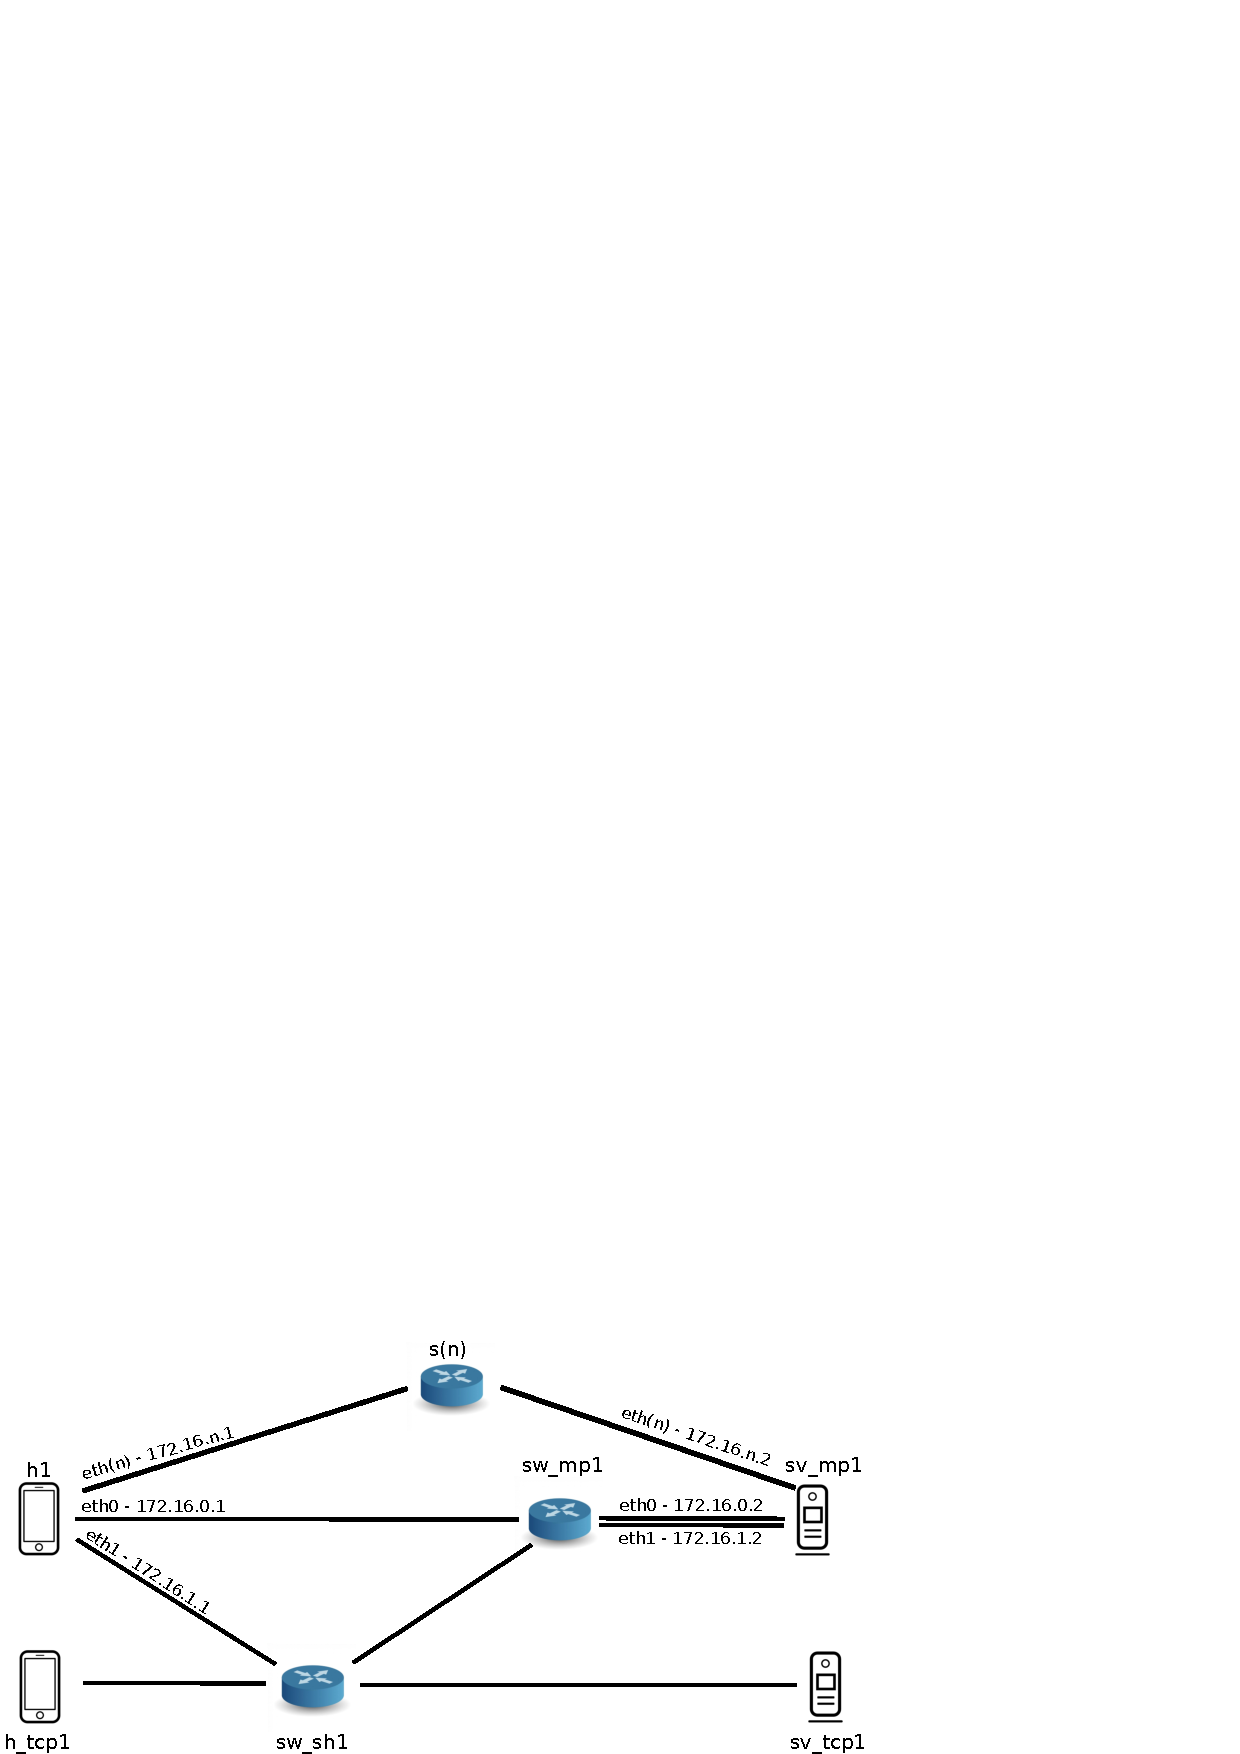
\includegraphics[width=0.7\textwidth]{../figures/mptcp_tcp/mptcp_tcp.pdf}
  \end{changemargin}
  \centering
  
  \caption{\textbf{Reproduction de la topologie de l'article de
      R. Khalili}. Le(s) \emph{switch(s)} n ne sont pr�sent(s) que si
    le nombre de sous-flot est sup�rieure � deux. Pour n sous-flots,
    il y aura n-2 \emph{switchs} en plus et autant de liens
    suppl�mentaires. L'hyperviseur est connect� � tous les
    switchs. Pour se connecter via ssh aux h�tes, un \emph{switch} \og
    root \fg est cr�� et est connect� au \emph{switch} sw\_mp1 voir
    utilisations CF linktobeadded.}
  \label{fig:topoMPTCP:inks}
  
\end{figure}




\subsection{Performance de MPTCP sur mininet}
\label{sec:CR:perfMPTCP:base}

Apr�s la compilation du noyau, pour v�rifier le fonctionnement de
MPTCP nous avons mesur� le d�bit moyen en utilisant \emph{iperf} sur
la topologie A.

Les param�tres\footnote{param�tres par d�faut dans le noyau Linux}
utilis�s sont les suivants:


\vspace{1cm}
%\begin{tabular}{lp{\linewidth - 4cm}} 
\begin{tabular}{ll}
  \textbf{Param�tre}& \textbf{Valeur}\\
  \hline
  MSS& 1460 octets\footnote{Une erreur se produit lorsque nous fixons la valeur voir \pref{sec:annexe1:bugs:mininet}}\\
  window size& 85,3 Koctets\\
  d�lai par lien & 10 ms\\
  Algorithme de congestion& LIA \cite{rfc6356}\\
\end{tabular}
\vspace{0.5cm}


\subsubsection{Un exemple de d�monstration}
\label{sec:CR:perfMPTCP:unique}

Nous allons prendre, dans cet exemple, une connexion avec deux
sous-flots avec une capacit� individuelle de 100 Mbit/s. Voici la
commande pour g�n�rer cet exemple:
\begin{verbatim}
sudo python ./pyMPTCP -O exp001_TC --bw 100 -t 30 -n 2 --mptcp --bwm_ng
\end{verbatim}

Pour les d�tails de l'activation de MPTCP dans le noyau et
l'utilisation des arguments des scripts python, une notice est donn�e
en Annexe 1: voir sections \ref{sec:annexe1:usepyth} page
\pageref{sec:annexe1:usepyth} et \ref{sec:annexe1:mininetParserargs}
page \pageref{sec:annexe1:mininetParserargs}.

\vspace{0.5cm} Le RTT entre h1 et sv\_mp1 est de 44\,$\pm$\,11\,ms
(mesur� avec la commande \emph{ping}), ce qui correspond au RTT
attendu pour traverser deux liens aller-retour. La moyenne ici tient
compte du RTT du premier paquet qui est envoy� vers le contr�leur pour
que celui-ci �tablisse le chemin vers le serveur.

L'argument ``-\,-bwm\_ng'' permet de lancer Bandwidth Monitor
NG\footnote{\url{http://www.gropp.org/?id=projects&sub=bwm-ng} }
(bwm-ng). Cette application mesure plusieurs param�tres: le nombre
d'octets, de paquets, le d�bit entrant ou sortant passant par chacune
des interfaces de l'h�te sond�. La figure \ref{fig:MPTCP-perfbwm-ng}
repr�sente le d�bi entrant enregistr� au serveur pour ses deux
interfaces. Nous observons pour deux sous-flots aux capacit�s
identiques et au co�t identique, que le d�bit mesur� est quasi
similaire (une diff�rence de quelques paquets est observ�e).

\begin{figure}[htb]
    \centering
    \includegraphics[width=0.7\textwidth]{../figures/bw-single.pdf}
    \caption{\textbf{D�bit entrant c�t� serveur.} �chantillonage : 2\,Hz.}
  \label{fig:MPTCP-perfbwm-ng}
\end{figure}

Pour mesurer le d�bit total g�n�r�, nous effectuons une moyenne des
d�bits totaux mesur�s toutes les secondes par \emph{iperf} entre 5
secondes apr�s le d�but de la connexion, et 1 seconde avant la fin de
la connexion. Nous observons pour cet exemple, c�t� serveur, un d�bit
maximal de 168\,Mbit/s. Ce d�bit est coh�rent par rapport aux mesures
de d�bit \emph{via} bwm-ng.


\subsubsection{Variation du d�bit maximal par lien}
\label{sec:CR:perfMPTCP:nsousflots}

Pour conna�tre les limites de nos simulations, nous avons fait varier
la capacit� de chaque sous-flot, ainsi que le nombre de sous-flots
dans la topologie A.

\begin{figure}[htb]
    \centering
    \includegraphics[width=0.7\textwidth]{../figures/bw-coupled.pdf}
    \caption{\textbf{D�bit total mesur� en fonction de la capacit� du
        sous-flot.} Les d�bits sont mesur�s avec \emph{iperf} pour une
      connexion TCP classique et une connexion MPTCP contenant de 2 �
      6 sous-flots.}
  \label{fig:MPTCP-perf-subflow-bw}
\end{figure}

Le d�bit totale mesur� au serveur cro�t lin�airement avec
l'augmentation du nombre de sous-flots pour des capacit�s par lien de
10 � environ 100\,Mbit/s. Cette phase est en ad�quation avec le but de
MPTCP : augmentation des performances \cite{rfc6182}. Cependant, pour
les liens aux capacit�s sup�rieures � 100\,Mbit/s, les performances
d�croissent rapidement et tombent en dessous des performances d'une
simple connexion TCP ce qui viole la nature m�me de MPTCP .

Ce probl�me pourrait �tre expliqu� par une utilisation non optimale
de la capacit� des sous-flots. Le \emph{bandwidth delay product} (BDP)
implique une taille minimale du tampon de r�ception. Pour un d�bit de
1000\,Mo et un RTT de 44\,ms, la taille minimale du tampon est de
5,5\,Mo. Sachant que le tampon de r�ception\footnote{dans notre
  simulation la taille des tampons de r�ception est la m�me que la
  taille des tampons d'envoi.}  est partag� pour tous les sous-flots
d'une connexion MPTCP, la taille minimale du tampon doit suivre cette
formule \cite{rfc6824} :

\begin{equation}
  \label{eq:MPTCP:buffer}
  buffer\_size \geqslant max(\{RTT_i\}_{i \in [1,n]})*\sum_{i \in [1,n]} Bandwidth_{\{i\}}
\end{equation}

C'est � dire que la taille du tampon de r�ception doit �tre sup�rieure
ou �gal au produit du RTT le plus �lev� parmi tous les sous-flots et
la somme des capacit�s de tous les sous-flots. Cette taille de tampon
garantit l'utilisation optimale du lien lorsque des paquets
n�cessitent d'�tre retransmisent sur des sous-flots aux d�lais
lents. Dans notre simulation, il n'y a pas de perte de paquets, la
valeur minimale des tampons correspond au BDP le plus �lev�.

Pour les m�mes propri�t�s de liens, avec deux sous-flots, nous
obtenons une taille minimale de 11\,Mo. Mininet modife automatiquement
les tampons au lancement de la topologie et les valeurs utilis�es sont
les suivantes (en octets):

\begin{verbatim}
net.core.wmem_max = 16777216
net.core.wmem_default = 163840
net.core.rmem_max = 16777216
net.core.rmem_default = 163840
net.ipv4.tcp_wmem = 10240	87380	16777216
net.ipv4.tcp_rmem = 10240	87380	16777216
net.ipv4.tcp_mem = 19326	25768	38652
\end{verbatim}

Nous observons que le tampon maximal pouvant �tre allou� par socket
est de 16\,Mo environ ce qui est largement sup�rieur � la taille
requise. De plus en augmentant la taille du tampon, nous n'observons
pas d'augmentation de performances alors qu'en le diminuant, nous
observons une diminution du d�bit mesur� (voir
Fig. \ref{fig:mptcp:windowscale}).

\begin{figure}[!htb]
    \includegraphics[width=0.7\textwidth]{../figures/ws.pdf}
    \centering
    \caption{\textbf{D�bit mesur� en fonction de la taille de la
        fen�tre}. La taille maximmale de la fen�tre TCP est modifi�e
      avec l'argument '-w' avec \emph{iperf}. La taille obtenue est
      �trangement deux fois sup�rieure � la taille demand�. Le nombre
      de paquets indiqu� dans la l�gende correspond � la capacit� de
      traitement, en nombre de paquets, des routeurs.}
  \label{fig:mptcp:windowscale}
  
\end{figure}

Nous obtenons les m�mes r�sultats en modifiant la capacit� des
routeurs ou en modifiant les valeurs de la taille des tampons dans le
noyau (voir \ref{sec:annexe1:windowsize} page
\pageref{sec:annexe1:windowsize}) que ce soit les param�tres minimum,
par d�faut et maxium d'\emph{auto-tuning} de TCP (\emph{net.ipv4}) ou
les valeurs maximales ou par d�faut pour tous les type de connexions
(\emph{net.core}). Une v�rification de la charge CPU global avec
\emph{htop} ne montre pas une saturation des processeurs (environ
15\,\% d'utilisation) cependant, il reste � impl�menter \emph{cpuacct}
pour v�rifier la charge CPU par conteneur.


En effectuant des
recherches\footnote{\url{https://github.com/mininet/mininet/wiki/Introduction-to-Mininet\#what-are-mininets-limitations}}\footnote{\url{https://mailman.stanford.edu/pipermail/mininet-discuss/2014-January/003901.html}},
il semblerait que la limite du d�bit est li� aux n\oe uds Open vSwitch
sur Ubuntu 13.04, ce qui pour une dizaine de liens, limite la capacit�
maximale � environ 100 Mbit/s. De plus, il semblerait que l'activation
de \emph{auto-tuning} pour les tailles des tampons entra�nent une
basse significative des performances de MPTCP \cite{PKB13}. C'est pourquoi,
nous limiterons la capacit� des liens � de faibles valeurs.

\subsubsection{Variation du d�lai par lien}
\label{sec:compterendu:perf:d�lai}

Afin d'�valuer l'influence du d�lai sur le d�bit enregistr�, le d�lai
de tous les liens varie de mani�re sym�trique. Le co�t pour chaque
sous-flot reste donc identique.

Pour mesurer le d�lai de chaque sous-flot, nous avons utilis� la
commande \emph{ping}. Cette approche a �t� utilis�e car elle est la
plus facile � mettre en \oe uvre. Par manque d'espace disque (m�moire
SSD), l'utilisation de \emph{tcpdump} est r�serv�e pour les tests et
la recherche d'erreur. Cependant, il sera n�cessaire d'utiliser le
d�lai avec TCP car cette m�thode est plus fiable et l'utilisation
conjointe de \emph{ping} et d'\emph{iperf} produit une erreur (voir
\pref{sec:annexe1:bugs:mininet}).\\


\begin{figure}[tb]
    \centering
    \includegraphics[width=0.7\textwidth]{../figures/rtt.pdf}
  \centering
  
  \caption{\textbf{D�bit maximal mesur� en fonction du d�lai}. Le
    d�lai est du m�me ordre de grandeur pour tous les liens. Le RTT
    est mesur� avec la commande \emph{ping} avant le test avec
    \emph{iperf} qui dure 60\,s. Deux sous-flots sont utilis�s.}
  \label{fig:mptcp:rttisotrop}
  
\end{figure}

Nous observons que la modification du d�lai n'entra�ne pas de
diminution des performances pour les liens � faibles capacit�s
\fig{fig:mptcp:rttisotrop}. Ce qui est attendu vu que la taille des
\emph{buffers} et la capacit� des routeurs sont largement suffisantes
pour satisfaire � une augmentation de d�bit. Il reste alors � tester
ces cas dans des
conditions plus stringentes.\\

Pour les liens � haute capacit�, l'augmentation de d�lai entra�ne une
diminution du d�bit total. Pour 200\,Mbit/s et 400\,ms de RTT, il est
n�cessaire d'avoir environ 10\,Mo de tampon par sous-flot. Cependant,
il est possible que cette diminution drastique pour le lien �
200\,Mbit/s est en partie li�e aux probl�mes de simulation des d�bits
�l�v�s
avec mininet.\\


Nous constatons que la taille du tampon s'av�re �tre un param�tre
primordial dans les performances de MPTCP. Dans une utilisation
mobile, les deux sous-flots ont g�n�ralement des d�lais diff�rents
(par exemple, si on se base sur l'utilisation conjointe d'un acc�s
wifi, 3G ou/et ethernet). Dans la figure \ref{fig:mptcp:rttetTC}, nous
utilisons les m�mes param�tres que dans l'exp�rience pr�c�dente
cependant le premier sous-flot aura le m�me RTT (une dizaine de
millisecondes) pour toutes les exp�riences (exp�riences ``TC''). Nous
n'observons aucune diff�rence notable entre le cas o� les deux
sous-flots ont un RTT variable et dans le cas o� un seul des
sous-flots poss�de un RTT variable. L'exp�rience ``200 TC'' montre que
le d�bit est plus �lev� que l'exp�rience ``200'', cette diff�rence
peut �tre expliquer par une taille du tampon insuffisante.



\begin{figure}[htb]
    \includegraphics[width=0.7\textwidth]{../figures/prefixtc.pdf}
  \centering
  \caption{\textbf{D�bit total mesur� en fonction du d�lai d'un
      lien}. Le d�lai est modifi�e seulement pour le second lien dans
    la topologie A (exp�riences ``TC''). Le RTT est mesur� avec la
    commande \emph{ping} avant le test avec \emph{iperf} qui dure
    60\,s. Deux sous-flots sont utilis�s.}
  \label{fig:mptcp:rttetTC}
\end{figure}

\subsubsection{Choix du sous-flot en fonction du d�lai}
\label{sec:compterendu:perf:5choix}


Pour tester quels sont les sous-flots choisies par MPTCP dans une
connexion � \og faible \fg d�bit. Nous avons utilis� 5 sous-flots avec
diff�rents RTT. Le RTT de chaque sous-flot suit une sigmo�de (�quation
\ref{eq:sigmoide}).

\begin{equation}
  \label{eq:sigmoide}
  delay=min+\frac{max}{1+e^{\frac{x-x_{half}}{slope}}}
\end{equation}

Les param�tres\footnote{slope et $x_{half}$ ne sont pas utiles et
  permettent de contraindre le nombre d'exp�riences et la courbure des
  points d'inflexion.} utilis�s sont les suivants:

\vspace{1cm}
%\begin{tabular}{lp{\linewidth - 4cm}} 
\begin{tabular}{ll}
\textbf{Param�tre}& \textbf{Valeur}\\
\hline
delay& d�lai par lien\\
max& d�lai maximal par lien\\
min& d�lai minimal par lien\\
\end{tabular}
\vspace{0.5cm}

\begin{figure}[H]
    \includegraphics[width=0.7\textwidth]{../figures/TC5.pdf}
  \centering
  \caption{\textbf{D�bit re�u par interface c�t� serveur en fonction
      du RTT par sous-flot}. \emph{En haut}, RTT pour chaque
    sous-flot. \emph{Au milieu}, d�bit (Mbit/s) par interface. En bas,
    d�bit total (Mbit/s) enregistr� au serveur.}
  \label{fig:mptcp:sigmoid}
\end{figure}

Nous observons que le d�bit re�u est globalement �quivalent pour
chaque interface sauf pour l'interface ``eth4'' o� son d�bit est
inf�rieur � celles des autres pour des RTTs sup�rieur � 300\,ms. Le
d�bit total n'est que faiblement diminu�. En effet, la commande
\emph{iperf} envoie des paquets jusqu'� atteindre la capacit� de
chaque sous-flot. La l�g�re diminution des d�bits pour les d�lais long
est probablement
li�e au tampon de r�ception ou d'envoi.\\

Il est donc difficile de pr�dire les sous-flots utilis�s par
l'ordonnanceur. \emph{iperf} ne permet de contraindre le d�bit que
pour des paquets UDP. Nous avons donc int�gr�
\emph{iperf3\footnote{\url{https://github.com/esnet/iperf}}} � la VM
mininet
pour permettre de fixer le d�bit pour des paquets TCP.\\

L'utilisation d'\emph{iperf3} entra�ne une erreur qui n'a pas �t�
encore r�solue � la fin de la simulation (voir
\pref{sec:annexe1:bugs:mininet}) emp�chant toutes simulations
automatis�es. Nous avons donc choisi deux r�sultats caract�ristiques.

\begin{figure}[H]
    \includegraphics[width=0.7\textwidth]{../figures/bw-5_1_5_10_100_500.pdf}
  \centering
  \caption{\textbf{D�bit mesur� pour chaque interface}. Les RTTs pour
    les interfaces de eth0 � eth5 sont de 34, 38, 43, 137,
    552\,ms. Chaque lien a une capacit� de 10\,Mbit/s et le d�bit
    total g�n�r� par \emph{iperf3} a �t� fix� � 7,5\,Mbit/s.  }
  \label{fig:mptcp:bw151050}
\end{figure}

Dans la figure \ref{fig:mptcp:bw151050} et
\ref{fig:mptcp:bw1010500500500} nous observons que MPTCP envoie
pr�f�rentiellement les paquets dans les sous-flots � faible RTT. Il
�quilibre les charges dans les sous-flots o� le d�lai reste
raisonnable (sous-flot � RTT de 147\,ms dans la figure
\ref{fig:mptcp:bw151050}. Cependant pour les sous-flots � \og co�ts
\fg identiques, nous observons un effet de battement
(\emph{flappiness}). Il serait utile de mesurer le RTT au cours du
temps pour chaque sous-flot et d'�tablir si cet effet de battement est
li� � une variation du d�lai et ce pour l'algorithme LIA et OLIA
\cite{pareto2013}.

\begin{figure}[H]
    \includegraphics[width=0.7\textwidth]{../figures/bw-5_10_10_500_500_500.pdf}
  \centering
  \caption{\textbf{D�bit mesur� pour chaque interface}. Les RTTs pour
    les interfaces de eth0 � eth5 sont de 43, 43, 557, 557,
    557\,ms. Chaque lien a une capacit� de 10\,Mbit/s et le d�bit
    total g�n�r� par \emph{iperf3} a �t� fix� � 7,5\,Mbit/s.  }
  \label{fig:mptcp:bw1010500500500}
\end{figure}





\clearpage


%// -*- coding: iso-8859-1 -*-

\section{Annexe}
\label{sec:annexe1:annexe1}

\input{section/annexe1/scripts}

\subsection{Bugs}
\label{sec:annexe1:mininetClass}

\subsubsection{Topologie}
\label{sec:annexe1:bugs:topo}

\`A la cr�ation de la topologie mininet, il est n�cessaire de donner
des noms courts aux h�tes et aux switchs.\\

Il n'est pas possible de cr�er deux liens entre les m�mes n\oe uds de
la classe ``Topo''. Pour contourner cette limitation, il faut cr�� la
topologie avec un seul lien puis dans la classe ``Mininet'', rajouter
le second lien. C'est pourquoi, dans le fichier
``\emph{pyMPTCP\_topo.py}'', il y a deux d�finitions pour la m�me
topologie: une pour la classe Topo (\emph{topo()}) et une autre pour
la classe Mininet (\emph{topo\_options(args,net)}) qui sera execut�
s�quentiellement lors de la simulation.\\


\subsubsection{mininet}
\label{sec:annexe1:bugs:mininet}

\paragraph{iperf et ping}
L'utilisation conjointe de la commande \emph{iperf} et de la commande
ping dans une simulation produit une erreur du calcul du d�lai par la
commande ping. Ce d�lai augmente exponentiellement vers environ
1000\,ms. Si on analyse les traces enregistr�s avec \emph{tcpdump},
les r�ponses aux \emph{echo request} se produisent bien plus
rapidement que ne laissent sug�rer les r�sultats de la commande
\emph{ping}. L'utilisation conjointe de ces deux applications marchent
tr�s bien entre la machine physique et la VM et il est probable que ce
probl�me soit li� � mininet.\\


\paragraph{MSS}
Lorsque nous fixons le \emph{Maximum Segment Size} � 1460 octets, nous
obtenons ce message d'erreur:
\begin{verbatim}
  WARNING: attempt to set TCP maximum segment size to 1460, but got
  536
\end{verbatim}

Cependant, si nous analysons les paquets enregistr�s gr�ce �
\emph{tcpdump}, nous observons que le MSS n�goci� pendant le
\emph{handshake} de la connexion est bien de 1460 octets et que la
taille des paquets de donn�es est de 1428 octets.

\paragraph{iperf3}
Dans l'�tat des scripts, \emph{Iperf3} produit une erreur � la fin de
la simulation. Il est n�cessaire de nettoyer la simulation et il n'est
pas possible pour l'instant d'utiliser les scripts \emph{shell} pour
effectuer des simulations automatis�es.

\begin{verbatim}
sudo bash shMPTCP.sh clean
\end{verbatim}





%\subsection{Exp�riences}
%\label{sec:annexe1:experiment}
%
Description des fichiers pythons dans le dossier experiment\\




TCPvsMPTCP$/$ \\
\hspace*{2cm}\lunder init\lunder.py\\
\hspace*{2cm}pyMPTCP.py\\
\hspace*{2cm}\textbf{experiment}/\\
\hspace*{4cm}\lunder init\lunder.py\\
\hspace*{4cm}experiment.py\\
\hspace*{4cm}experiment001\_TC.py\\
\hspace*{4cm}\ldots\\






\begin{tabular}{lp{\linewidth - 4cm}}

\textbf{fichier}& \textbf{Commentaires}\\
\hline
experiment.py&  fixe d�lai h1-eth1, valeur � modifier dans le fichier\\
exp001_TC.py&  fixe d�lai h1-eth1, valeur � modifier dans le fichier\\

\end{tabular}



\bibliography{./PRES}
\bibliographystyle{ieeetr}



\label{fin} %% Ne pas supprimer, n�cessaire pour calculer le nombre de pages RL
\end{document}


%%% Local Variables: 
%%% mode: latex
%%% TeX-master: t
%%% End: 
